\documentclass[11pt]{article}
\usepackage[a4paper,margin=1in]{geometry}
\usepackage{fontspec}
\setmainfont{Noto Serif CJK SC}
\setsansfont{Noto Sans CJK SC}
\setmonofont{Latin Modern Mono}
\XeTeXlinebreaklocale "zh"
\XeTeXlinebreakskip = 0pt plus 1pt
\usepackage{amsmath,amssymb,amsthm,mathtools}
\usepackage{booktabs,longtable,array,multirow}
\usepackage{enumitem}
\usepackage{graphicx}
\usepackage{xcolor}
\usepackage{float}
\usepackage{hyperref}
\usepackage{tikz}
\usepackage{pgfplots}
\usetikzlibrary{arrows.meta,positioning,shapes.geometric,calc,fit}
\pgfplotsset{compat=1.18}
\hypersetup{colorlinks=true,linkcolor=blue!50!black,urlcolor=blue!50!black}
\renewcommand{\contentsname}{目录}
\renewcommand{\figurename}{图}
\renewcommand{\tablename}{表}

\title{DEO 分割与量化方法\\算法、数学定义与指标总表}
\author{Lachlan Chen}
\date{2026-04-05}

\newcommand{\R}{\mathbb{R}}
\newcommand{\1}{\mathbf{1}}
\newcommand{\dx}{\,\mathrm{d}x}
\newcommand{\IoU}{\operatorname{IoU}}
\newcommand{\ovsmall}{\operatorname{ov}_{\mathrm{small}}}
\newcommand{\clip}{\operatorname{clip}}
\newcommand{\med}{\operatorname{median}}
\newcommand{\mean}{\operatorname{mean}}
\newcommand{\std}{\operatorname{std}}
\newcommand{\sem}{\operatorname{sem}}
\newcommand{\quantile}{\operatorname{Q}}
\newcommand{\dilate}{\operatorname{dilate}}
\newcommand{\erode}{\operatorname{erode}}
\newcommand{\openop}{\operatorname{open}}
\newcommand{\closeop}{\operatorname{close}}
\newcommand{\dist}{\operatorname{dist}}
\newcommand{\symdiff}{\triangle}
\newcommand{\normminmax}{\mathcal{N}}
\newcommand{\support}{M_{\mathrm{sup}}}
\newcommand{\unionmask}{U}
\newcommand{\edgefield}{E}
\newcommand{\signal}{S}
\newcommand{\gray}{I}
\newcommand{\labelmap}{L}

\begin{document}
\maketitle
\tableofcontents

\section{范围}
本文档系统说明 DEO 项目中当前使用的分割与量化框架，主要覆盖以下已完成的分析流程：
\begin{itemize}[leftmargin=1.5em]
  \item App80：Y-27632 浓度实验；
  \item App65：alginate 浓度实验；
  \item App81：接种密度实验。
\end{itemize}

本文的目标是把以下内容放在同一个可复查的技术说明中：
\begin{itemize}[leftmargin=1.5em]
  \item 分割算法本身；
  \item hybrid signal 图像及 support mask 的构造；
  \item multiscale Cellpose 与大质量不规则结构恢复分支；
  \item 候选掩膜的评分与合并逻辑；
  \item 所有下游量化指标的数学定义。
\end{itemize}

本文给出的是仓库中\textbf{全部已实现指标的并集}。并不是每个数据集都会用到全部指标，但下面的公式覆盖了当前项目中完整的指标族。

\section{符号约定}
设图像定义域为 $\Omega \subset \mathbb{Z}^2$，原始明场灰度图像为
\begin{equation}
\gray: \Omega \to [0,255].
\end{equation}
若原始 TIFF 为 RGB，则先经 RGB 转灰度后得到 $\gray$。

设最终实例标签图为
\begin{equation}
\labelmap: \Omega \to \{0,1,2,\dots,K\},
\end{equation}
其中标签 $0$ 表示背景，$K$ 表示该图像中的类器官实例数。

对任一实例 $k \in \{1,\dots,K\}$，定义其二值区域为
\begin{equation}
\Omega_k = \{x \in \Omega : \labelmap(x)=k\}.
\end{equation}

其实例几何量定义为：
\begin{align}
A_k &= |\Omega_k| && \text{像素面积},\\
P_k &= \text{实例 } \Omega_k \text{ 的周长},\\
c_k &= \text{实例 } \Omega_k \text{ 的质心}.
\end{align}

所有实例的并集定义为
\begin{equation}
\unionmask = \bigcup_{k=1}^{K} \Omega_k.
\end{equation}

\section{流程总览}
\subsection{高层流程图}
\begin{figure}[H]
\centering
\begin{tikzpicture}[
  node distance=7mm and 9mm,
  box/.style={draw, rounded corners, align=center, minimum height=8mm, text width=27mm, fill=blue!4},
  box2/.style={draw, rounded corners, align=center, minimum height=8mm, text width=27mm, fill=green!4},
  box3/.style={draw, rounded corners, align=center, minimum height=8mm, text width=27mm, fill=orange!7},
  arrow/.style={-Latex, thick}
]
\node[box] (tif) {原始 TIFF\\明场图像};
\node[box, right=of tif] (gray) {灰度化\\与基础标准化};
\node[box2, right=of gray] (signal) {Hybrid signal 图像\\黑背景强化图};
\node[box2, below=of signal] (support) {Support mask\\由 signal 阈值获得};
\node[box3, right=of signal] (cellpose) {Cellpose 多尺度分支\\$d_1,d_2,d_3$};
\node[box3, below=of cellpose] (recover) {Signal 恢复分支\\连通域 + watershed};
\node[box, right=of recover] (merge) {候选评分\\与重叠感知合并};
\node[box, right=of merge] (out) {保存输出\\mask, overlay, signal,\\JSON, CSV};

\draw[arrow] (tif) -- (gray);
\draw[arrow] (gray) -- (signal);
\draw[arrow] (signal) -- (cellpose);
\draw[arrow] (signal) -- (support);
\draw[arrow] (signal) -- (recover);
\draw[arrow] (support) -- (merge);
\draw[arrow] (cellpose) -- (merge);
\draw[arrow] (recover) -- (merge);
\draw[arrow] (merge) -- (out);
\end{tikzpicture}
\caption{DEO 分割流程的高层结构。}
\end{figure}

\subsection{指标依赖关系图}
\begin{figure}[H]
\centering
\begin{tikzpicture}[
  node distance=8mm and 10mm,
  src/.style={draw, rounded corners, align=center, minimum height=8mm, text width=28mm, fill=gray!10},
  grp/.style={draw, rounded corners, align=center, minimum height=8mm, text width=34mm, fill=purple!6},
  arrow/.style={-Latex, thick}
]
\node[src] (raw) {原始灰度图 $\gray$};
\node[src, right=of raw] (sig) {Hybrid signal $\signal$};
\node[src, right=of sig] (lab) {标签图 $\labelmap$};

\node[grp, below left=12mm and -4mm of raw] (growth) {生长指标\\count, area, perimeter,\\signal-sum 趋势};
\node[grp, below=12mm of sig] (fusion) {融合指标\\edge, curvature,\\internal-edge, center-weighted};
\node[grp, below right=12mm and -4mm of lab] (diff) {分化指标\\roundness, darkness,\\wall/core morphology};

\draw[arrow] (raw) -- (growth);
\draw[arrow] (sig) -- (growth);
\draw[arrow] (sig) -- (fusion);
\draw[arrow] (lab) -- (growth);
\draw[arrow] (lab) -- (fusion);
\draw[arrow] (lab) -- (diff);
\draw[arrow] (raw) -- (diff);
\end{tikzpicture}
\caption{各类指标分别依赖哪些中间数据产品。}
\end{figure}

\section{分割算法}
\subsection{Hybrid signal 图像}
保存下来的黑背景 signal 图像，是整个流程中最关键的预处理表示之一。它既用于 support 区域提取，也用于大量下游指标计算。

记经 CLAHE 增强后的灰度图为
\begin{equation}
\tilde{I} = \operatorname{CLAHE}(\gray).
\end{equation}

再定义：
\begin{align}
F &= G_{\sigma_f} * \tilde{I} && \text{小核前景模糊},\\
B &= G_{\sigma_b} * \tilde{I} && \text{大核背景模糊},\\
R &= B - F && \text{背景减前景后的 residual},\\
V &= 255 - F && \text{前景反相图像}.
\end{align}

记将图像 min-max 归一化到 $[0,255]$ 的操作为 $\normminmax(\cdot)$。最终 hybrid signal 定义为
\begin{equation}
\signal = 0.45\,\normminmax(V) + 0.55\,\normminmax(R).
\end{equation}

当前代码中，典型固定参数为：
\begin{itemize}[leftmargin=1.5em]
  \item CLAHE clip limit $=2.4$；
  \item 前景 Gaussian blur kernel $=3\times3$；
  \item 背景 Gaussian blur kernel $=31\times31$。
\end{itemize}

\subsection{Support mask}
为了得到一个具备生物学支持意义的前景区域，流程首先从 hybrid signal 中提取 support mask。阈值定义为
\begin{equation}
T_{\mathrm{sup}} = \max\left(T_{\mathrm{Otsu}}(\signal),\; \quantile_{0.58}(\signal)\right).
\end{equation}

对应的原始阈值掩膜为
\begin{equation}
M_{\mathrm{sup},0}(x)=\1[\signal(x)\ge T_{\mathrm{sup}}].
\end{equation}

再经过开运算和闭运算清理，得到最终 support mask：
\begin{equation}
\support = \closeop\bigl(\openop(M_{\mathrm{sup},0})\bigr).
\end{equation}

必须强调：support mask 不是最终分割结果。它只是一种支持先验，用来：
\begin{itemize}[leftmargin=1.5em]
  \item 细化 Cellpose 输出；
  \item 剔除支持度过弱的候选掩膜；
  \item 在后续恢复大而不规则结构时提供约束。
\end{itemize}

\subsection{Cellpose 多尺度分支}
与单一直径不同，该方法对每张图像同时评估多个候选直径：
\begin{equation}
\mathcal{D} = \{d_1,d_2,d_3\}.
\end{equation}

对每个 $d \in \mathcal{D}$，Cellpose 产生一个标签图：
\begin{equation}
\labelmap^{(d)} = \operatorname{Cellpose}(\gray; d).
\end{equation}

具体直径三元组是数据集相关、阶段相关的。在 App80 中，后期融合阶段使用的直径明显大于早期 cluster 阶段。

\subsection{梯度图与候选掩膜特征}
在代码中，会从 CLAHE 图像或 hybrid signal 图像计算梯度强度图。统一记归一化后的 edge map 为 $\edgefield(x)\in[0,1]$。

对任意候选掩膜 $\Omega_k$，主要候选特征定义如下。

\paragraph{Support ratio}
\begin{equation}
r_{\mathrm{sup},k} = \frac{|\Omega_k \cap \dilate(\support)|}{|\Omega_k|}.
\end{equation}

\paragraph{Mean signal}
\begin{equation}
\mu_{\signal,k} = \frac{1}{|\Omega_k|}\sum_{x\in\Omega_k} \frac{\signal(x)}{255}.
\end{equation}

\paragraph{Boundary edge strength}
设 $\partial \Omega_k$ 表示候选掩膜的形态学边界，则
\begin{equation}
e_{\partial,k} = \frac{1}{|\partial \Omega_k|}\sum_{x\in\partial \Omega_k} \edgefield(x).
\end{equation}

\paragraph{Bounding-box fill ratio}
若 $\Omega_k$ 的轴对齐包围盒宽高分别为 $w_k$ 和 $h_k$，则
\begin{equation}
f_{\mathrm{box},k} = \frac{A_k}{w_k h_k}.
\end{equation}

\paragraph{Circularity}
\begin{equation}
\chi_k = \frac{4\pi A_k}{P_k^2}.
\end{equation}

\subsection{候选评分}
候选掩膜的分数由多个生物学上有意义的分量加权组成：
\begin{equation}
s_k = 1.85\,r_{\mathrm{sup},k} + 0.85\,\mu_{\signal,k} + 0.65\,e_{\partial,k} + 0.25\,f_{\mathrm{box},k} + b_{\mathrm{stage}} + b_{\mathrm{branch}}.
\end{equation}

其中：
\begin{itemize}[leftmargin=1.5em]
  \item $b_{\mathrm{stage}}$ 是与阶段相关的加分项；
  \item $b_{\mathrm{branch}}$ 是对不同候选分支的轻微偏置项。
\end{itemize}

这些 bonus 都是经验性的。它们的作用是让评分更贴合已知形态阶段，例如早期 cluster、囊泡阶段、后期大面积融合结构等。

\subsection{基于 signal 的大质量结构恢复}
Cellpose 单独使用时，最常见的失败模式之一是漏掉非常大且形状不规则的融合结构。为此，流程还会直接对 hybrid signal 做阈值分割。

对给定分位数 $q$，定义阈值后的 signal 掩膜：
\begin{equation}
B_q(x) = \1[\signal(x) \ge \quantile_q(\signal)].
\end{equation}

随后对其进行闭运算、开运算、清除边缘、填孔，并提取连通域。

第二条恢复路径使用距离变换生成 watershed seeds。定义
\begin{equation}
D_q(x) = \dist(B_q)(x),
\end{equation}
并通过
\begin{equation}
Z_q(x) = \1\left[D_q(x) > \tau \max_{y\in\Omega} D_q(y)\right]
\end{equation}
生成种子，再在阈值区域内运行 watershed，以得到更多大结构候选。

\subsection{候选合并逻辑}
最终的实例集合由所有分支候选通过重叠感知合并得到。

对两个掩膜 $A$ 与 $B$，定义：
\begin{align}
\IoU(A,B) &= \frac{|A\cap B|}{|A\cup B|},\\
\ovsmall(A,B) &= \frac{|A\cap B|}{\min(|A|,|B|)}.
\end{align}

实际代码逻辑可概括为：
\begin{itemize}[leftmargin=1.5em]
  \item 若 $\ovsmall>0.80$ 或 $\IoU>0.60$，则将两者视作对同一结构的竞争解释；
  \item 若新的候选具有明显更高分数，或在支持度不明显变差的前提下拥有更合理的大面积，则替换旧候选；
  \item 若一个小碎片与已接受的大掩膜明显重叠，则丢弃该碎片。
\end{itemize}

\subsection{保存输出}
每张图像最终会保存以下结果：
\begin{itemize}[leftmargin=1.5em]
  \item \texttt{*\_mask\_16bit.png}：16 位实例标签图；
  \item \texttt{*\_instance\_rgb.png}：随机颜色实例图；
  \item \texttt{*\_overlay.png}：原图与实例叠加图；
  \item \texttt{*\_signal.png}：hybrid signal 图像；
  \item \texttt{*\_metrics.json}：每图量化指标；
  \item \texttt{*\_segmentation\_stats.json}：分割来源和分支统计信息。
\end{itemize}

\section{几何与空间基础量}
\subsection{距离变换与 centrality}
对任一实例 $\Omega_k$，定义其内部的欧氏距离变换为
\begin{equation}
D_k(x) = \dist(\Omega_k)(x), \qquad x\in\Omega_k.
\end{equation}

归一化 centrality 场定义为
\begin{equation}
C_k(x) = \frac{D_k(x)}{\max_{y\in\Omega_k} D_k(y)} \in [0,1].
\end{equation}

因此：
\begin{itemize}[leftmargin=1.5em]
  \item 边界附近的像素满足 $C_k(x)\approx 0$；
  \item 最深内部区域满足 $C_k(x)=1$。
\end{itemize}

\subsection{指数型中心权重}
为了更强地强调实例内部的边缘信号，定义 centrality 权重函数：
\begin{equation}
w_{\alpha}(c)=\frac{e^{\alpha c}-1}{e^{\alpha}-1}, \qquad c\in[0,1].
\end{equation}

当前实现使用 $\alpha=5$。

\begin{figure}[H]
\centering
\begin{tikzpicture}
\begin{axis}[
  width=0.72\textwidth,
  height=0.36\textwidth,
  xlabel={中心性 $c$},
  ylabel={$w_{\alpha}(c)$},
  xmin=0, xmax=1,
  ymin=0, ymax=1.02,
  domain=0:1,
  samples=200,
  grid=both,
  thick
]
\addplot[blue!70!black] {(exp(5*x)-1)/(exp(5)-1)};
\addplot[dashed,gray] {x};
\legend{$w_{5}(c)$, 线性参考}
\end{axis}
\end{tikzpicture}
\caption{center-weighted internal-edge 系列指标所使用的指数中心权重。}
\end{figure}

\subsection{Wall/core 分解}
在分化相关的 darkness 指标中，每个类器官实例会被拆分为 wall 区与 core 区。

若实例面积为 $A_k$，其等效半径定义为
\begin{equation}
r_k^{\mathrm{eq}} = \sqrt{\frac{A_k}{\pi}}.
\end{equation}

对应的侵蚀厚度定义为
\begin{equation}
t_k = \clip\left(\operatorname{round}(0.12\,r_k^{\mathrm{eq}}), 5, 30\right).
\end{equation}

于是：
\begin{align}
\Omega_k^{\mathrm{core}} &= \erode(\Omega_k; t_k),\\
\Omega_k^{\mathrm{wall}} &= \Omega_k \setminus \Omega_k^{\mathrm{core}}.
\end{align}

\begin{figure}[H]
\centering
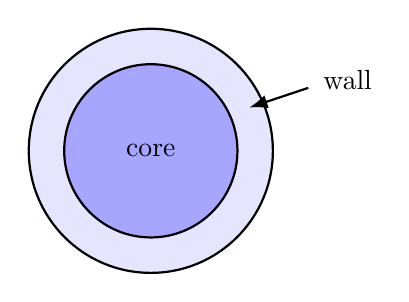
\begin{tikzpicture}[scale=1.0]
\fill[blue!10] (0,0) circle (1.55);
\fill[blue!35] (0,0) circle (1.10);
\draw[thick] (0,0) circle (1.55);
\draw[thick] (0,0) circle (1.10);
\node at (0,0) {core};
\node at (2.5,0.9) {wall};
\draw[-Latex,thick] (2.0,0.8) -- (1.25,0.55);
\end{tikzpicture}
\caption{用于 darkness 指标的自适应 wall/core 分解示意。}
\end{figure}

\section{指标定义}
本节给出当前 DEO 工作流中全部已实现指标的统一数学定义。

\subsection{生长指标}
\paragraph{Count}
\begin{equation}
N = K.
\end{equation}
表示单张图像中的分割实例数。

\paragraph{Total segmented area}
\begin{equation}
A_{\mathrm{tot}} = \sum_{k=1}^{K} A_k.
\end{equation}
这是目前最核心的基于分割的生长指标之一。

\paragraph{Average perimeter}
\begin{equation}
\bar{P} = \frac{1}{K}\sum_{k=1}^{K} P_k,
\end{equation}
并约定当 $K=0$ 时取 $\bar{P}=0$。

\paragraph{Signal sum intensity}
Hybrid signal 的总强度定义为
\begin{equation}
I_{\mathrm{sum}} = \sum_{x\in\Omega} \signal(x).
\end{equation}
它是一个探索性的形态敏感强度代理量。

\paragraph{Reciprocal signal sum}
\begin{equation}
I_{\mathrm{sum}}^{-1} = \frac{1}{I_{\mathrm{sum}}}.
\end{equation}
当反比形式更容易解释趋势时会使用该指标。

\paragraph{Signal sum relative change}
对时间点 $t$，定义
\begin{equation}
\Delta_{\mathrm{sum}}^{\mathrm{rel}}(t) = \frac{I_{\mathrm{sum}}(t)-I_{\mathrm{sum}}(t-1)}{I_{\mathrm{sum}}(t-1)}.
\end{equation}

\paragraph{Reciprocal signal sum relative change}
\begin{equation}
\Delta_{\mathrm{recip}}^{\mathrm{rel}}(t) = \frac{I_{\mathrm{sum}}^{-1}(t)-I_{\mathrm{sum}}^{-1}(t-1)}{I_{\mathrm{sum}}^{-1}(t-1)}.
\end{equation}

\subsection{融合指标：边界与形状核心指标}
\paragraph{Boundary edge intensity}
设 $B_{\partial}$ 为所有实例边界像素的并集，则
\begin{equation}
E_{\partial} = \frac{1}{|B_{\partial}|}\sum_{x\in B_{\partial}} \edgefield(x).
\end{equation}
该指标对应 \texttt{edge\_intensity}。

\paragraph{Per-instance circularity}
对单个实例，定义
\begin{equation}
\chi_k = \frac{4\pi A_k}{P_k^2}.
\end{equation}
这就是标准的面积-周长 circularity。

\paragraph{Image-level curvature}
项目中的 curvature 指标，定义为 circularity 的面积加权平均：
\begin{equation}
C = \frac{1}{A_{\mathrm{tot}}}\sum_{k=1}^{K} A_k\chi_k.
\end{equation}
它对应 \texttt{curvature}。

\paragraph{带下限的 min-max 归一化}
对任意逐图像标量 $v_i$，定义
\begin{equation}
\operatorname{norm}_{\eta}(v_i) = \max\left(\eta, \frac{v_i-v_{\min}}{v_{\max}-v_{\min}}\right),
\end{equation}
其中当前实现取 $\eta=0.1$，$v_{\min},v_{\max}$ 在当前批次内计算。

据此得到：
\begin{align}
N_{\mathrm{norm}} &= \operatorname{norm}_{0.1}(N),\\
C_{\mathrm{norm}} &= \operatorname{norm}_{0.1}(C),\\
E_{\mathrm{norm}} &= \operatorname{norm}_{0.1}(E_{\partial}).
\end{align}

\paragraph{Normalized edge over count and curvature}
\begin{equation}
M_{\mathrm{norm}} = \frac{E_{\mathrm{norm}}}{N_{\mathrm{norm}}\,C_{\mathrm{norm}}}.
\end{equation}
它对应 \texttt{normalized\_edge\_over\_count\_curvature}。

\paragraph{Inverse edge-count-curvature product}
\begin{equation}
M_{\mathrm{inv}} = \frac{1}{E_{\partial}\,N\,C}.
\end{equation}
它对应 \texttt{inverse\_edge\_count\_curvature}。

\paragraph{Edge density}
设 $T$ 为根据原始亮场 residual 构建的 tissue mask，$B_E$ 为模糊灰度图上的 Canny 边缘集合，则
\begin{equation}
\rho_E = \frac{|B_E \cap T|}{|T|}.
\end{equation}
该指标对应 \texttt{edge\_density}。

\paragraph{Reciprocal edge density}
\begin{equation}
\rho_E^{-1} = \frac{1}{\max(\rho_E,\varepsilon)},
\end{equation}
其中 $\varepsilon$ 为数值稳定项。

\paragraph{Gradient mean}
若 $G_x,G_y$ 为 Sobel 导数，且 $G=\sqrt{G_x^2+G_y^2}$，则
\begin{equation}
\bar{G}_T = \frac{1}{|T|}\sum_{x\in T} G(x).
\end{equation}
该指标对应 \texttt{gradient\_mean}。

\paragraph{Reciprocal gradient mean}
\begin{equation}
\bar{G}_T^{-1} = \frac{1}{\max(\bar{G}_T,\varepsilon)}.
\end{equation}

\subsection{融合指标：internal-edge 与空间再分布}
这一类指标直接对应项目中的核心假设：融合增强时，边缘结构会从类器官外缘向内部迁移。

\paragraph{Central inside edge mean}
利用 centrality $C_k(x)$ 定义：
\begin{equation}
E_{\mathrm{cen}} = \frac{\sum_{k=1}^{K}\sum_{x\in\Omega_k} \edgefield(x)\,C_k(x)}{\sum_{k=1}^{K}\sum_{x\in\Omega_k} C_k(x)}.
\end{equation}
它对应 \texttt{central\_inside\_edge\_mean}。

\paragraph{Peripheral inside edge mean}
\begin{equation}
E_{\mathrm{per}} = \frac{\sum_{k=1}^{K}\sum_{x\in\Omega_k} \edgefield(x)\,(1-C_k(x))}{\sum_{k=1}^{K}\sum_{x\in\Omega_k} (1-C_k(x))}.
\end{equation}
它对应 \texttt{peripheral\_inside\_edge\_mean}。

\paragraph{Outer-ring edge mean}
定义外环区域为
\begin{equation}
R_{\mathrm{out}} = \dilate(\unionmask) \setminus \unionmask.
\end{equation}
则
\begin{equation}
E_{\mathrm{out}} = \frac{1}{|R_{\mathrm{out}}|}\sum_{x\in R_{\mathrm{out}}} \edgefield(x).
\end{equation}
它对应 \texttt{outer\_ring\_edge\_mean}。

\paragraph{Central inside fraction}
\begin{equation}
F_{\mathrm{cen}} = \frac{E_{\mathrm{cen}}}{E_{\mathrm{cen}}+E_{\mathrm{per}}}.
\end{equation}
它对应 \texttt{central\_inside\_fraction}。

\paragraph{Central / peripheral ratio}
\begin{equation}
R_{\mathrm{cen/per}} = \frac{E_{\mathrm{cen}}}{E_{\mathrm{per}}}.
\end{equation}
它对应 \texttt{central\_inside\_over\_peripheral}。

\paragraph{Central / outer ratio}
\begin{equation}
R_{\mathrm{cen/out}} = \frac{E_{\mathrm{cen}}}{E_{\mathrm{out}}}.
\end{equation}
它对应 \texttt{central\_inside\_over\_outer}。

\paragraph{Peripheral / central ratio}
\begin{equation}
R_{\mathrm{per/cen}} = \frac{E_{\mathrm{per}}}{E_{\mathrm{cen}}}.
\end{equation}
它对应 \texttt{peripheral\_over\_central}。

\paragraph{Center-weighted edge sum}
使用指数型权重 $w_{\alpha}$，定义
\begin{equation}
S_{\mathrm{cw}} = \sum_{k=1}^{K}\sum_{x\in\Omega_k} \edgefield(x)\,w_{\alpha}(C_k(x)).
\end{equation}
它对应 \texttt{center\_weighted\_edge\_sum}。

\paragraph{Center-weighted edge weight sum}
\begin{equation}
W_{\mathrm{cw}} = \sum_{k=1}^{K}\sum_{x\in\Omega_k} w_{\alpha}(C_k(x)).
\end{equation}
它对应 \texttt{center\_weighted\_edge\_weight\_sum}。

\paragraph{Center-weighted edge mean}
\begin{equation}
\bar{E}_{\mathrm{cw}} = \frac{S_{\mathrm{cw}}}{W_{\mathrm{cw}}}.
\end{equation}
它对应 \texttt{center\_weighted\_edge\_mean}。

\paragraph{Mean instance center-weighted edge sum}
若单个实例的 center-weighted edge sum 为
\begin{equation}
S_{\mathrm{cw},k}=\sum_{x\in\Omega_k} \edgefield(x)\,w_{\alpha}(C_k(x)),
\end{equation}
则其实例平均值定义为
\begin{equation}
\bar{S}_{\mathrm{cw,inst}} = \frac{1}{K}\sum_{k=1}^{K} S_{\mathrm{cw},k}.
\end{equation}
它对应 \texttt{instance\_center\_weighted\_edge\_sum\_mean}。

\paragraph{Area-normalized center-weighted edge}
对每个实例定义
\begin{equation}
a_k = \frac{S_{\mathrm{cw},k}}{A_k}.
\end{equation}
则保存的三个统计量为：
\begin{align}
\bar{a} &= \frac{1}{K}\sum_{k=1}^{K} a_k && \texttt{area\_normalized\_center\_weighted\_edge\_instance\_mean},\\
\std(a_k) &&& \texttt{area\_normalized\_center\_weighted\_edge\_instance\_std},\\
\operatorname{median}(a_k) &&& \texttt{area\_normalized\_center\_weighted\_edge\_instance\_median}.
\end{align}

\subsection{分化指标：几何 roundness}
这组指标用于衡量分割实例与同面积参考圆之间的偏离程度。

\paragraph{Reference circle}
对实例 $\Omega_k$，其质心为 $c_k$，面积为 $A_k$，定义同面积半径：
\begin{equation}
r_k = \sqrt{\frac{A_k}{\pi}}.
\end{equation}
相应参考圆定义为
\begin{equation}
\Gamma_k = \{x\in\Omega : \|x-c_k\|_2 \le r_k\}.
\end{equation}

\paragraph{Absolute area deviation from reference circle}
\begin{equation}
D_k = |\Omega_k \symdiff \Gamma_k|.
\end{equation}
这就是目标实例与参考圆的对称差面积，单位为像素。

\paragraph{Normalized deviation}
\begin{equation}
\delta_k = \frac{D_k}{|\Omega_k \cup \Gamma_k|}.
\end{equation}
它对应对象级别的 \texttt{roundness\_deviation\_norm}。

\paragraph{Roundness}
\begin{equation}
R_k = \max(0, 1-\delta_k).
\end{equation}
这就是对象级别的 roundness 分数。

\paragraph{Image-level roundness}
\begin{equation}
R = \frac{1}{A_{\mathrm{tot}}}\sum_{k=1}^{K} A_k R_k.
\end{equation}
它对应图像级别的 \texttt{roundness}。

\paragraph{Image-level normalized deviation}
\begin{equation}
\delta = \frac{1}{A_{\mathrm{tot}}}\sum_{k=1}^{K} A_k\delta_k.
\end{equation}
它对应图像级别的 \texttt{roundness\_deviation\_norm}。

\paragraph{Total deviation pixels}
\begin{equation}
D_{\mathrm{tot}} = \sum_{k=1}^{K} D_k.
\end{equation}
它对应 \texttt{roundness\_deviation\_px\_total}。

\subsection{分化指标：darkness 与 wall thickening}
这组指标主要针对分化增强时更深、更厚、更暗的上皮壁及 budding 结构。

\paragraph{Background grayscale median}
设背景区域为膨胀后的实例并集补集：
\begin{equation}
B = \Omega \setminus \dilate(\unionmask).
\end{equation}
其背景中位灰度为
\begin{equation}
b = \med\{\gray(x): x\in B\}.
\end{equation}
它对应 \texttt{background\_gray\_median}。

\paragraph{Normalized darkness field}
相对于背景中位灰度，定义 darkness 场：
\begin{equation}
D(x) = \clip\left(\frac{b-\gray(x)}{\max(b,1)}, 0, 1\right).
\end{equation}
因此图像中越暗、相对背景越深的像素，其 $D(x)$ 越大。

\paragraph{Organoid darkness mean}
\begin{equation}
\bar{D}_{\unionmask} = \frac{1}{|\unionmask|}\sum_{x\in\unionmask} D(x).
\end{equation}
它对应 \texttt{organoid\_darkness\_mean}。

\paragraph{Organoid darkness upper quantiles}
\begin{align}
D_{0.90} &= \quantile_{0.90}\{D(x):x\in\unionmask\},\\
D_{0.95} &= \quantile_{0.95}\{D(x):x\in\unionmask\}.
\end{align}
它们分别对应 \texttt{organoid\_darkness\_p90} 与 \texttt{organoid\_darkness\_p95}。

\paragraph{Very dark area ratio}
固定阈值取 $\tau_D=0.35$，定义
\begin{equation}
R_{\mathrm{dark}>0.35} = \frac{|\{x\in\unionmask : D(x) > 0.35\}|}{|\unionmask|}.
\end{equation}
它对应 \texttt{very\_dark\_area\_ratio\_gt035}。

\paragraph{Wall darkness mean}
定义 wall 并集为
\begin{equation}
\unionmask^{\mathrm{wall}} = \bigcup_{k=1}^{K} \Omega_k^{\mathrm{wall}}.
\end{equation}
则
\begin{equation}
\bar{D}_{\mathrm{wall}} = \frac{1}{|\unionmask^{\mathrm{wall}}|}\sum_{x\in\unionmask^{\mathrm{wall}}} D(x).
\end{equation}
它对应 \texttt{wall\_darkness\_mean}。

\paragraph{Wall darkness 90th percentile}
\begin{equation}
D_{\mathrm{wall},0.90} = \quantile_{0.90}\{D(x): x\in\unionmask^{\mathrm{wall}}\}.
\end{equation}
它对应 \texttt{wall\_darkness\_p90}。

\paragraph{Core darkness mean}
定义 core 并集为
\begin{equation}
\unionmask^{\mathrm{core}} = \bigcup_{k=1}^{K} \Omega_k^{\mathrm{core}}.
\end{equation}
则
\begin{equation}
\bar{D}_{\mathrm{core}} = \frac{1}{|\unionmask^{\mathrm{core}}|}\sum_{x\in\unionmask^{\mathrm{core}}} D(x).
\end{equation}
它对应 \texttt{core\_darkness\_mean}。

\paragraph{Wall/core darkness ratio}
\begin{equation}
R_{\mathrm{wall/core}} = \frac{\bar{D}_{\mathrm{wall}}}{\max(\bar{D}_{\mathrm{core}}, 10^{-6})}.
\end{equation}
它对应 \texttt{wall\_core\_darkness\_ratio}。

\paragraph{Pixel-count bookkeeping}
另外还保存以下像素数，用于后续检查与解释：
\begin{align}
N_{\mathrm{pix,organoid}} &= |\unionmask|,\\
N_{\mathrm{pix,wall}} &= |\unionmask^{\mathrm{wall}}|,\\
N_{\mathrm{pix,core}} &= |\unionmask^{\mathrm{core}}|.
\end{align}
它们分别对应 \texttt{organoid\_pixel\_count}、\texttt{wall\_pixel\_count}、\texttt{core\_pixel\_count}。

\section{按生物学问题解释指标}
\subsection{生长}
最核心的生长相关指标通常是：
\begin{itemize}[leftmargin=1.5em]
  \item $A_{\mathrm{tot}}$：总分割面积；
  \item $N$：实例数，但解释时需要结合融合背景；
  \item $I_{\mathrm{sum}}$ 及其时间变化量。
\end{itemize}

\subsection{融合}
最核心的融合相关指标通常是：
\begin{itemize}[leftmargin=1.5em]
  \item $M_{\mathrm{norm}} = E_{\mathrm{norm}}/(N_{\mathrm{norm}}C_{\mathrm{norm}})$；
  \item $M_{\mathrm{inv}} = 1/(E_{\partial}NC)$；
  \item $E_{\mathrm{cen}}/E_{\mathrm{per}}$；
  \item center-weighted internal-edge 系列指标。
\end{itemize}

这些指标的共同出发点是：融合增强时，边缘结构不再只停留在类器官外缘，而会向内部转移。

\subsection{分化}
最核心的分化相关指标通常是：
\begin{itemize}[leftmargin=1.5em]
  \item roundness 与 roundness deviation 系列；
  \item organoid darkness 的高分位数；
  \item very dark area ratio；
  \item wall darkness 及 wall/core darkness ratio。
\end{itemize}

这些指标共同对应更厚的上皮壁、更暗的外观、以及 budding 或不规则分化结构。

\section{当前实现中的关键常数}
\begin{table}[H]
\centering
\small
\begin{tabular}{@{}lll@{}}
\toprule
量 & 当前典型值 & 作用 \\
\midrule
Hybrid signal 前景模糊 & $3\times3$ Gaussian & 局部前景支持 \\
Hybrid signal 背景模糊 & $31\times31$ Gaussian & 背景估计 \\
Hybrid signal 混合权重 & $0.45, 0.55$ & 反相项与 residual 项融合 \\
Support 阈值分位数 & $0.58$ & support 下限 \\
归一化地板值 & $0.1$ & 复合指标稳定化 \\
Very dark 阈值 & $0.35$ & 深色区域比例 \\
Wall band 比例 & $0.12\,r_k^{\mathrm{eq}}$ & wall/core 划分 \\
Wall band 范围限制 & $5$ 到 $30$ px & 保证 wall/core 稳定 \\
中心权重指数 & $\alpha=5$ & 强化内部权重 \\
\bottomrule
\end{tabular}
\caption{当前代码中最重要的固定常数。}
\end{table}

\section{与仓库代码的对应关系}
本文描述的方法主要对应以下代码目录：
\begin{itemize}[leftmargin=1.5em]
  \item \texttt{analysis-tools/app80\_first\_replicate\_multiscale\_cellpose/}
  \item \texttt{analysis-tools/app65\_alginate\_multiscale\_cellpose/}
  \item \texttt{analysis-tools/app81\_density\_multiscale\_cellpose/}
\end{itemize}

本文给出的指标并集，与仓库中的项目级指标目录相对应：
\begin{itemize}[leftmargin=1.5em]
  \item \texttt{references/deo\_metric\_catalog\_growth\_fusion\_differentiation.md}
\end{itemize}

\section{总结}
整个 DEO 工作流可以理解为两层：
\begin{enumerate}[leftmargin=1.8em]
  \item 分割层：以 multiscale Cellpose 为主体，并加入 deterministic 的 signal-based 大结构恢复分支；
  \item 量化层：基于保存下来的 mask、signal 和原始灰度图，计算生长、融合和分化三大类指标。
\end{enumerate}

分割架构本身具有一定可迁移性，但直径配置、阶段映射和恢复阈值仍然是数据集相关的。相比之下，指标层的可迁移性更强，因为它主要依赖已经保存的标签图、hybrid signal 图以及原始灰度图。

\end{document}
